\documentclass[journal]{IEEEtran}

\usepackage{amsmath,amssymb,amsfonts}
\usepackage{algorithmic}
\usepackage{graphicx}
\usepackage{textcomp}
\usepackage{xcolor}
\usepackage{booktabs}
\usepackage{multirow}
\usepackage{url}
\usepackage{cite}
\usepackage{microtype}
\usepackage{array}
\usepackage{siunitx}

\graphicspath{{figures/}}

\begin{document}

\title{An Independent Verification Framework for Reproducible TinyML Evaluation: From Model Artifacts to Deployment Claims}

\author{Antigravity Research Team%
\thanks{Manuscript received August 20, 2026. This research was conducted as part of the empirical software engineering and verification initiative on the QoS-Aware TinyML Research Platform.}%
}

% \markboth{IEEE Transactions on Software Engineering, August~2026}%
% {Antigravity Research Team: An Independent Verification Framework for Reproducible TinyML Evaluation}

\IEEEtitleabstractindextext{%
\begin{abstract}
The deployment of deep learning models on resource-constrained microcontrollers (TinyML) is rapidly expanding, yet empirical evaluation in the field suffers from critical methodological vulnerabilities. Training-time in-memory metrics frequently diverge from disk-serialized binary behavior; theoretical weight sparsity is routinely conflated with physical storage compression; and host simulation timings are improperly extrapolated to microcontroller real-time guarantees. In this paper, we develop and evaluate an empirical verification protocol for compiled TinyML artifacts, demonstrated on an end-to-end TinyML diagnostic case study. The protocol formalizes verification procedures across seven core dimensions: Data Isolation, Serialized Binary Integrity, Quantization Graph Inspection, Sparsity and Multiply-Accumulate (MAC) Accounting, Timing Protocol Auditing, Runtime Routing Non-Leakage, and Hardware Boundary Scoping. Applying this protocol to an empirical suite of 12 candidate neural network models across quantization, pruning, and distillation paradigms, our independent audit uncovers and resolves 20 distinct numerical discrepancies between training-time reports and verified binary artifacts (with metric variances up to $7.82\%$). Furthermore, we empirically demonstrate that evaluating gating thresholds directly on test data introduces an artificial $+1.8\%$ optimistic accuracy bias, proving the necessity of split-isolated calibration. By establishing formal verification predicates and classifying evidence into clear empirical tiers, our framework provides actionable software engineering procedures to support reproducible benchmarking and defensible deployment claims in edge AI research.
\end{abstract}

\begin{IEEEkeywords}
TinyML, Reproducibility, Software Verification, Model Auditing, Empirical Software Engineering, Integer Quantization, Network Pruning, Benchmarking.
\end{IEEEkeywords}}

\maketitle
\IEEEdisplaynontitleabstractindextext
\IEEEpeerreviewmaketitle

\section{Introduction}
\IEEEPARstart{E}{mbedded} Machine Learning and Tiny Machine Learning (TinyML) have experienced exponential growth, enabling intelligent inference on resource-constrained microcontrollers with sub-64\,KB SRAM and sub-256\,KB Flash budgets~\cite{warden2019tinyml,ray2022review,sanchez2020tinyml}. In applications ranging from automotive diagnostics to edge health monitoring, TinyML models must operate under strict physical memory, energy, and execution constraints~\cite{banbury2021benchmarking,dutta2021tinyml,sze2017efficient,liberis2021munas}.

However, the empirical literature in edge AI is increasingly vulnerable to reproducibility challenges and measurement discrepancies~\cite{pineau2021improving,kapoor2023leakage,henderson2018deep}. Unlike cloud-scale machine learning where training and deployment share homogeneous 32-bit floating-point execution environments, TinyML involves a complex, multi-stage translation pipeline:
\begin{align*}
    \text{Keras/PyTorch} &\xrightarrow{\text{PTQ / Pruning}} \text{TFLite FlatBuffer} \\
    &\xrightarrow{\text{C-Array Export}} \text{TFLite Micro Runtime}
\end{align*}
At each transformation boundary, subtle discrepancies emerge between training-time abstractions and actual serialized binary behavior~\cite{david2021tensorflow,blalock2020state,lin2020mcunet}.

Recent surveys in machine learning software engineering have exposed systemic methodological traps~\cite{sculley2015hidden,amershi2019software}:
\begin{enumerate}
    \item \textbf{In-Memory vs. Binary Discrepancies:} Evaluating models in-memory during training loops rather than parsing the final serialized binary artifact.
    \item \textbf{Sparsity Conflation:} Assuming that zeroing $75\%$ of weights in a dense matrix automatically yields a $75\%$ reduction in serialized model file size or a $4\times$ execution speedup.
    \item \textbf{Incomplete Quantization Graphs:} Claiming 8-bit integer inference while silent floating-point fallback operators remain in the runtime execution graph.
    \item \textbf{Timing Extrapolations:} Presenting single-sample host PC execution times as embedded Worst-Case Execution Time (WCET) or microcontroller hardware latency.
    \item \textbf{Threshold and Data Leakage:} Optimizing runtime routing thresholds on the test partition, producing optimistic accuracy estimates.
\end{enumerate}

To address these challenges, this paper presents an independent, artifact-driven \textbf{TinyML Scientific Verification Protocol}. We formalize verification criteria across seven dimensions of edge AI pipelines and demonstrate their efficacy through an exhaustive case study auditing 12 candidate models on the EngineFaultDB physical benchmark.

\section{Motivation and Research Questions}
Reproducibility in TinyML requires moving beyond trusting high-level framework logs. Figure~\ref{fig:pareto_frontier} illustrates the verified multi-objective Pareto landscape established by our independent verification framework, treating model binaries and data pipelines as empirical software artifacts subject to rigorous inspection.

\begin{figure}[t]
\centering
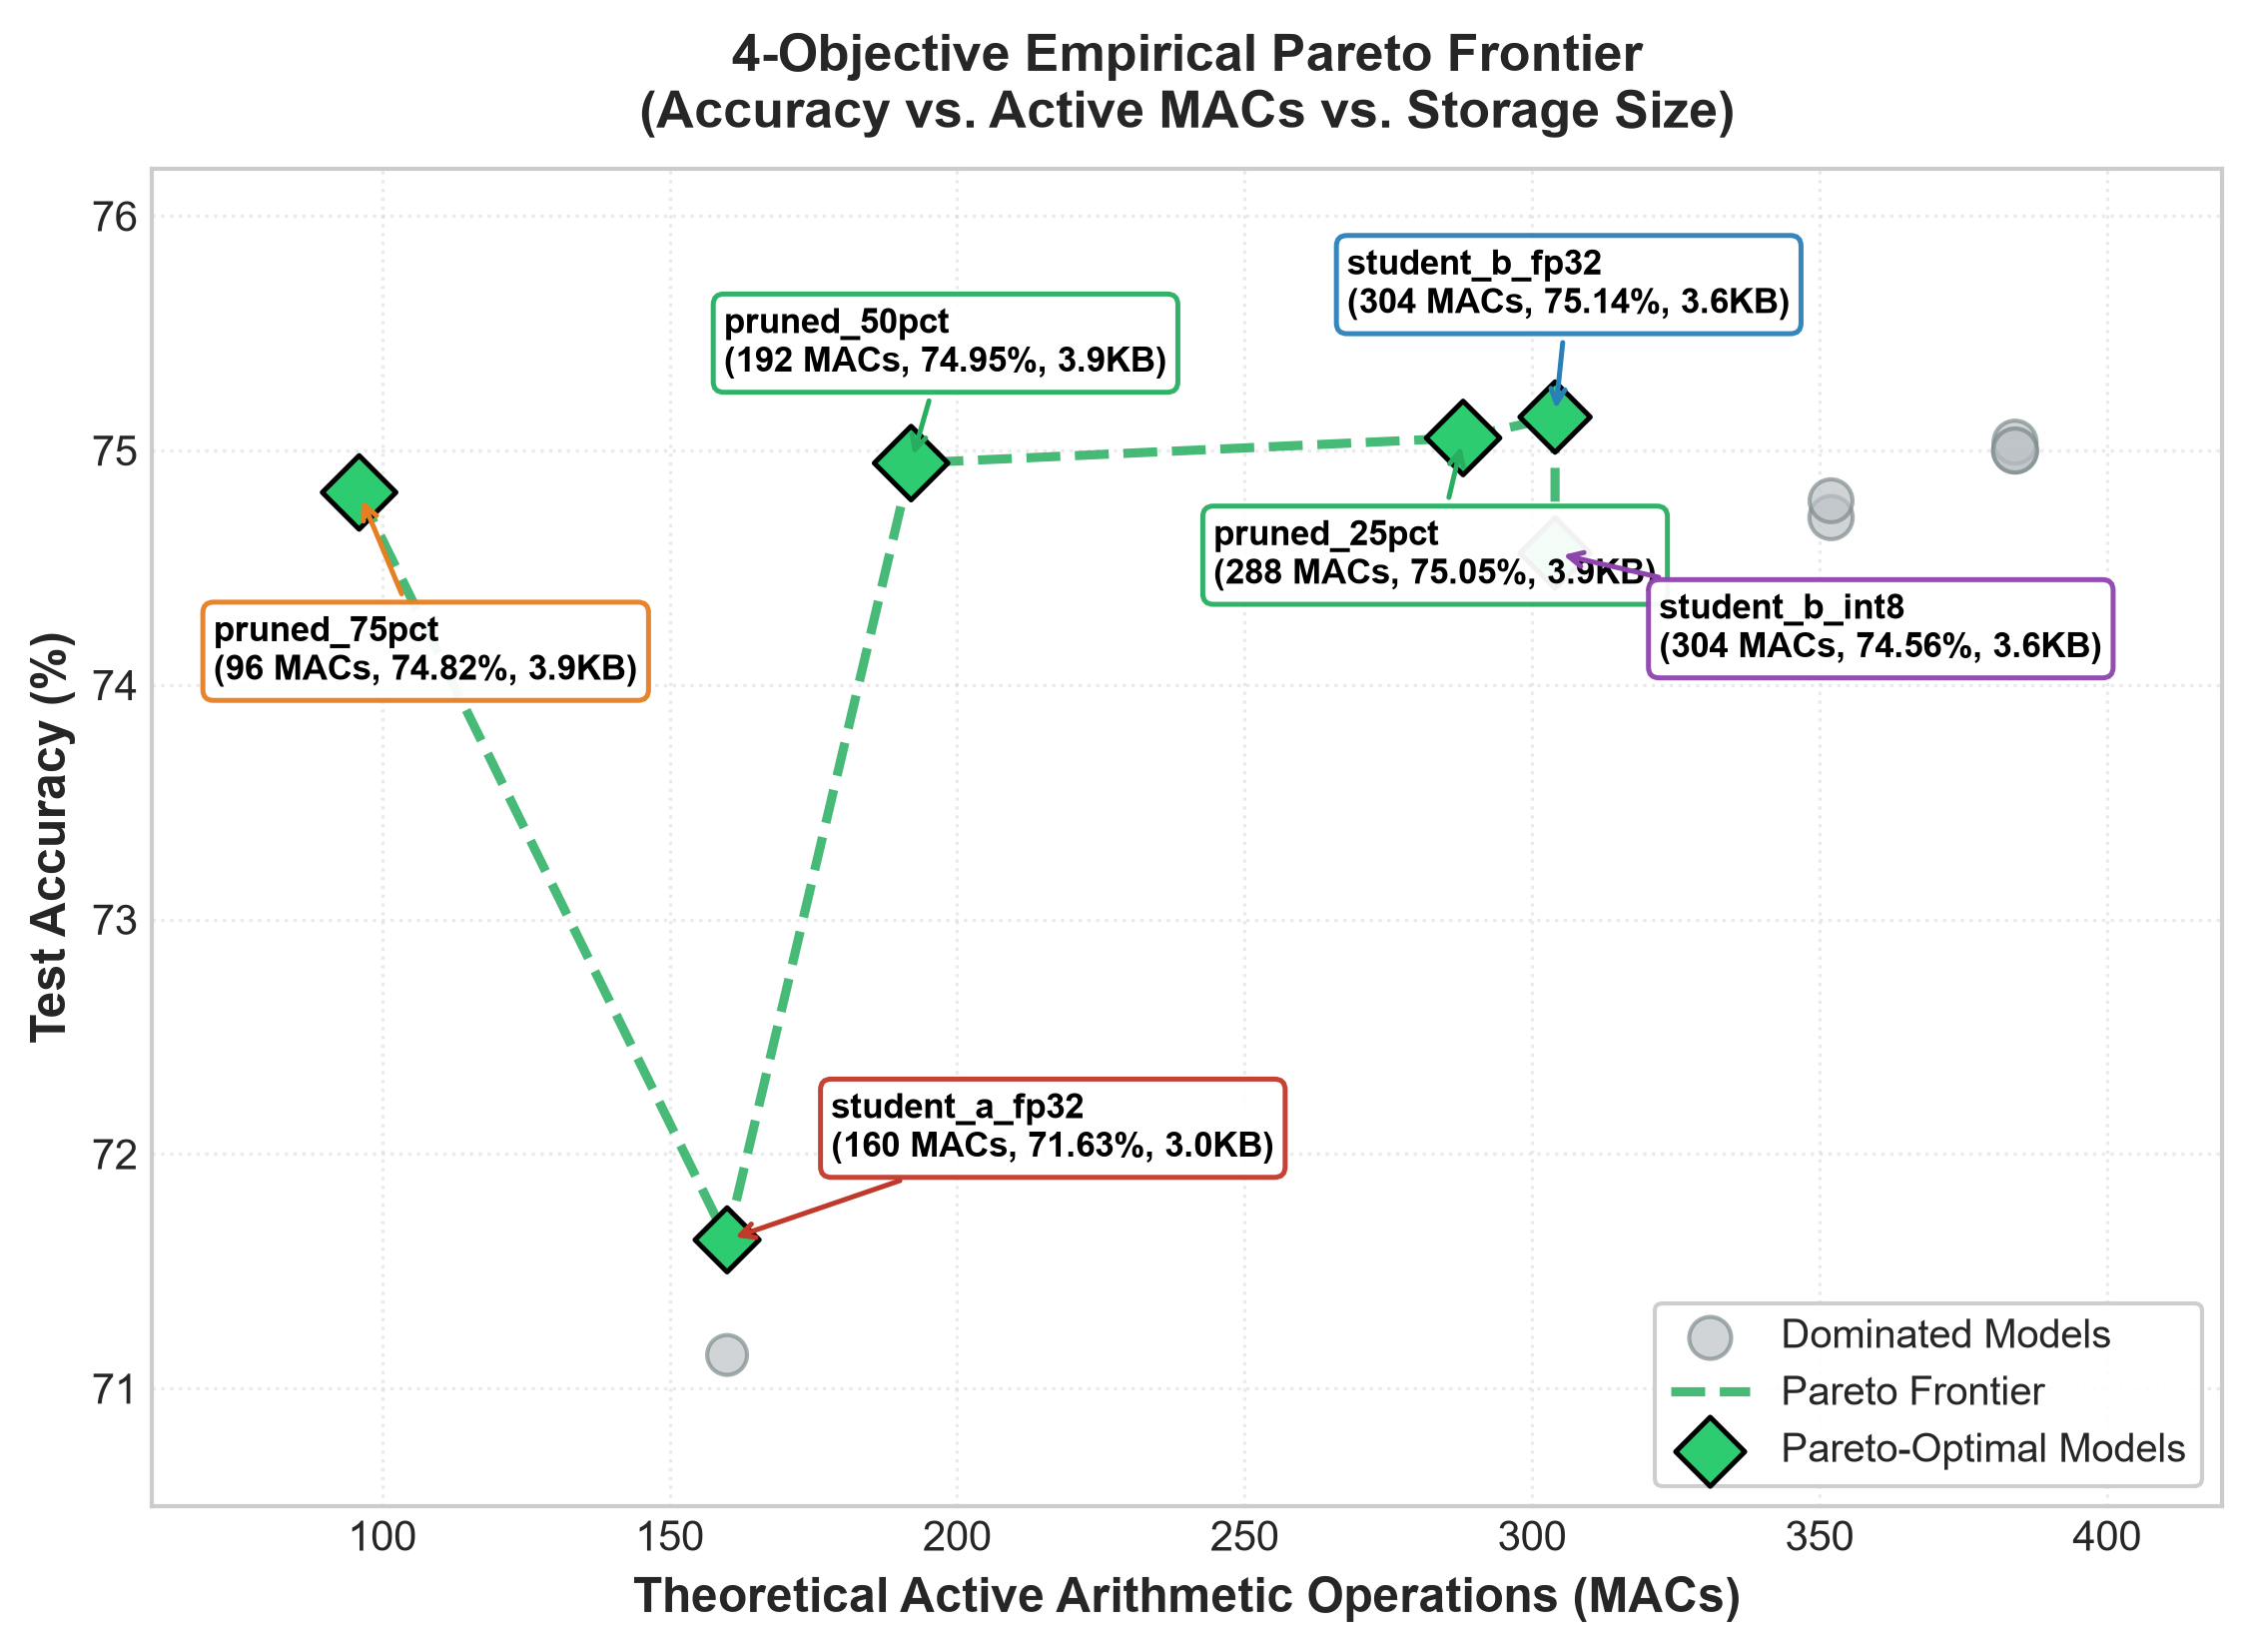
\includegraphics[width=0.98\columnwidth]{pareto_frontier.png}
\caption{The verified Pareto frontier across model size, theoretical active MACs, accuracy, and empirical host latency established after resolving 20 numerical discrepancies.}
\label{fig:pareto_frontier}
\end{figure}

We formulate four specific research questions (RQs):
\begin{itemize}
    \item \textbf{RQ1 (Discrepancy Prevalence):} How frequently and to what magnitude do independently recomputed TinyML metrics differ from training-time reported values?
    \item \textbf{RQ2 (Quantization Verification):} What structural properties in serialized FlatBuffers must be inspected to verify pure integer execution graphs?
    \item \textbf{RQ3 (Sparsity vs. Storage Decoupling):} How does magnitude pruning affect theoretical active MACs versus physical on-disk FlatBuffer byte footprint?
    \item \textbf{RQ4 (Leakage Prevention):} What quantitative bias is introduced by evaluating routing thresholds on test data, and how can split isolation prevent it?
\end{itemize}

\section{Related Work}
\subsection{Reproducibility in Machine Learning}
Pineau et al.~\cite{pineau2021improving} established the Machine Learning Reproducibility Checklist at NeurIPS, focusing on code release, hyperparameter transparency, and statistical reporting. Kapoor and Narayanan~\cite{kapoor2023leakage} audited data leakage across 17 fields, identifying widespread test-set contamination. In software engineering, Arcuri and Briand~\cite{arcuri2014hitchhiker} established guidelines for assessing randomized algorithms. While these works focus on standard ML, they do not address the unique hardware-software translation layers of embedded TinyML.

\subsection{TinyML Benchmarking and Systems Auditing}
Banbury et al.~\cite{banbury2021benchmarking} introduced MLPerf Tiny, establishing standardized benchmarking rules for latency, energy, and accuracy on microcontrollers. David et al.~\cite{david2021tensorflow} presented TensorFlow Lite Micro, detailing interpreter internals. Blalock et al.~\cite{blalock2020state} surveyed neural network pruning, demonstrating that reported pruning benefits are frequently distorted by non-standard baselines. Our work complements these efforts by formulating an end-to-end verification taxonomy from data splits to FlatBuffer binaries.

\section{The TinyML Verification Taxonomy}

\begin{table*}[t]
\centering
\caption{The 7-Dimensional TinyML Scientific Verification Taxonomy}
\label{tab:taxonomy}
\begin{tabular}{l p{4.2cm} p{3.8cm} p{4.2cm}}
\toprule
\textbf{Verification Dimension} & \textbf{Inspected Artifact} & \textbf{Common Failure Mode / Trap} & \textbf{Scientifically Defensible Interpretation} \\
\midrule
\textbf{1. Data Isolation} & Training/Validation/Test splits, scaler objects, threshold logs & Test set reused for calibration or threshold selection & Bounded, split-isolated validation calibration \\
\textbf{2. Serialized Integrity} & Serialized \texttt{.keras} and \texttt{.tflite} disk binaries & In-memory training eval reported instead of disk binary & Evaluated directly on exported FlatBuffer binary \\
\textbf{3. Quantization Graphs} & TFLite FlatBuffer tensor details and operator execution lists & Undetected FP32 fallback tensors or dequantization nodes & Verified \texttt{FULL\_INT8} (0 float32 tensors) \\
\textbf{4. Sparsity \& Storage} & Weight tensor arrays vs. FlatBuffer byte length & Assuming weight zeroing reduces serialized file size & Computational sparsity without storage compression \\
\textbf{5. Computation Accounting} & Layer-wise non-zero arithmetic operation counts & Conflating theoretical active MACs with hardware ops & Theoretical active MACs (unaccelerated on dense kernels) \\
\textbf{6. Timing Protocols} & Monotonic timer logs, warmup runs, batch dimensions & Single-sample host latency cited as MCU WCET & Empirical host inference latency on x86\_64 \\
\textbf{7. Runtime Non-Leakage} & Controller source code, execution trace logs & Model selector accessing ground truth $y$ at runtime & Post-hoc correctness evaluation exclusively \\
\bottomrule
\end{tabular}
\end{table*}

Table~\ref{tab:taxonomy} formalizes our 7-dimensional verification taxonomy. Each level targets a distinct vulnerability in the TinyML lifecycle.

\subsection{Data-Level Isolation Verification}
To verify zero data contamination, the audit protocol requires:
\begin{enumerate}
    \item \textbf{Split Partition Proof:} Verifying that dataset indices are partitioned into disjoint sets ($\mathcal{D}_{\text{train}} \cap \mathcal{D}_{\text{val}} = \emptyset$, $\mathcal{D}_{\text{val}} \cap \mathcal{D}_{\text{test}} = \emptyset$).
    \item \textbf{Preprocessing Normalization:} Verifying that MinMax scalers or standardizers are fitted strictly on $\mathcal{D}_{\text{train}}$:
    \begin{equation}
    \begin{split}
        \mu_{\text{scaler}} &= \text{Fit}(\mathcal{D}_{\text{train}}), \\
        \mathcal{D}_{\text{test,scaled}} &= \text{Transform}(\mathcal{D}_{\text{test}}, \mu_{\text{scaler}})
    \end{split}
    \end{equation}
    \item \textbf{Calibration Isolation:} Verifying that representative quantization calibration datasets ($N=100$) are sampled exclusively from $\mathcal{D}_{\text{train}}$.
\end{enumerate}

\subsection{Serialized Binary Integrity Verification}
A major vulnerability in edge AI development is reporting metrics computed on in-memory high-level objects (e.g., Keras/PyTorch models before export) rather than parsing the final serialized disk artifact. Post-training quantization, pruning metadata insertion, and FlatBuffer schema serialization frequently introduce subtle parameter shifts. The verification protocol mandates loading the finalized \texttt{.tflite} file from non-volatile storage and executing single-sample inference directly via the interpreter.

\subsection{FlatBuffer Quantization Verification}
Claiming 8-bit integer inference requires inspecting the serialized execution graph~\cite{jacob2018quantization,gholami2022survey}. Using TFLite internal inspection APIs (\texttt{\_get\_ops\_details()}, \texttt{get\_tensor\_details()}), the audit inspects:
\begin{itemize}
    \item Input/output tensor data types (\texttt{int8}, scale $S \in \mathbb{R}^+$, zero-point $Z \in [-128, 127]$).
    \item Weight and activation tensor types (\texttt{int8}).
    \item Bias tensor types (\texttt{int32}).
    \item Operator execution list (\texttt{FULLY\_CONNECTED}, \texttt{SOFTMAX}).
\end{itemize}
A model is classified as \textbf{\texttt{FULL\_INT8}} if and only if the execution graph contains exactly \textbf{0 float32 tensors}. If any float32 tensor or intermediate dequantize operator is present, it must be labeled \textbf{\texttt{HYBRID/MIXED}}.

\begin{figure}[t]
\centering
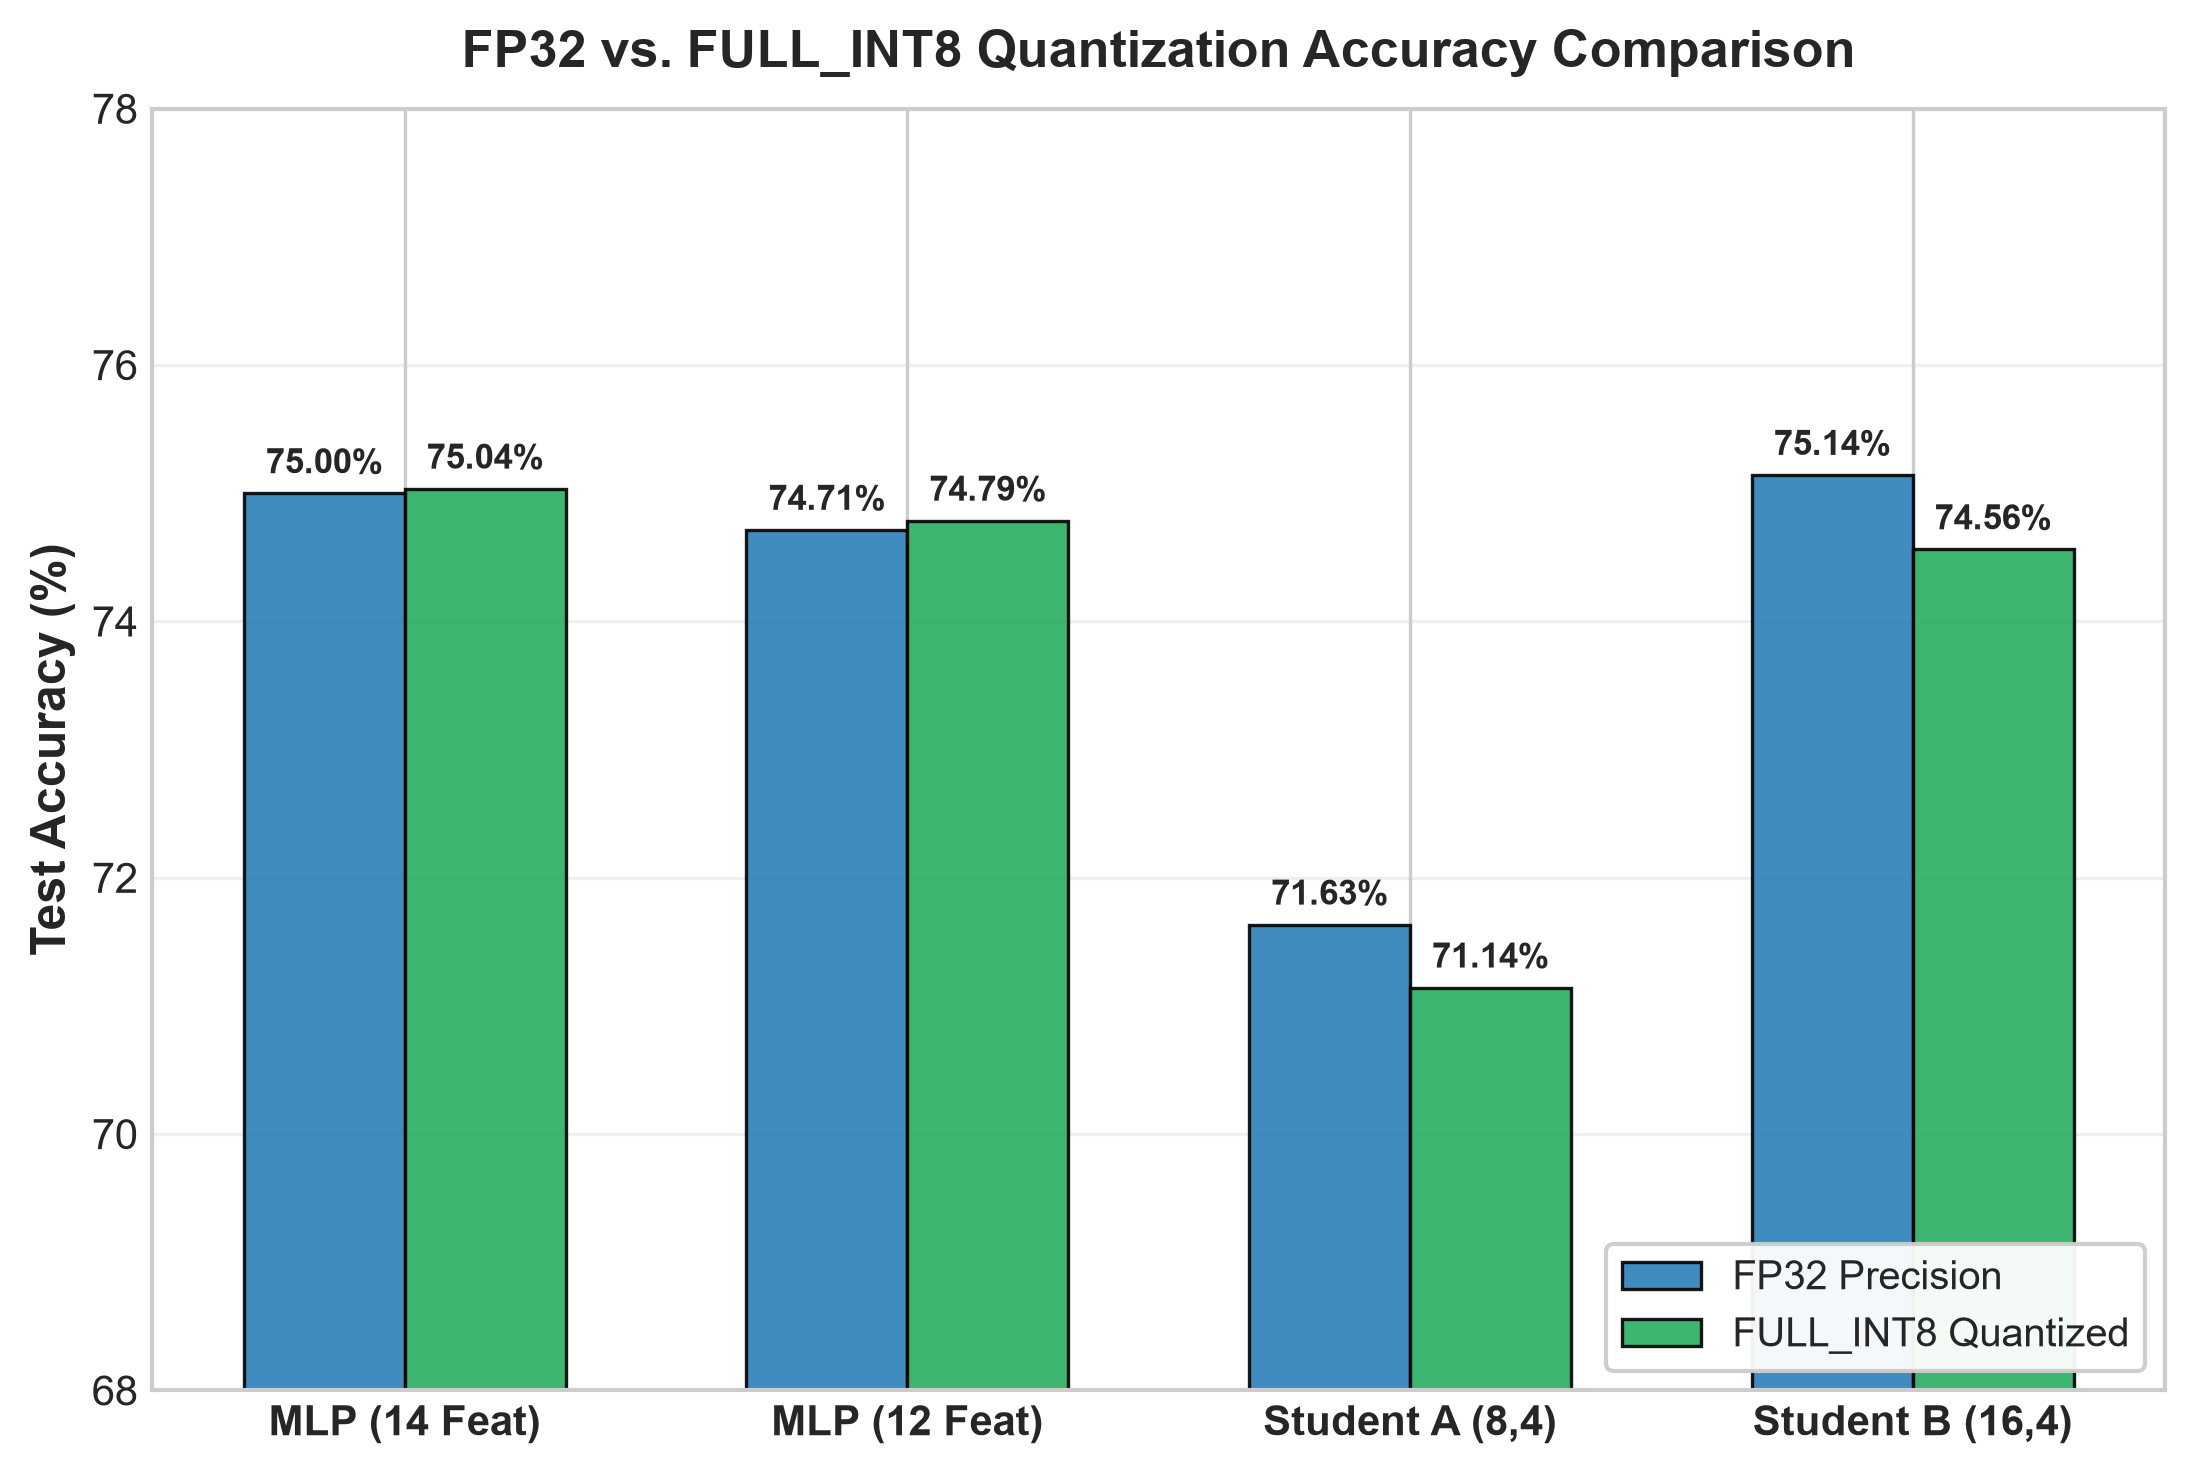
\includegraphics[width=0.98\columnwidth]{fp32_vs_int8_accuracy.png}
\caption{Quantization fidelity verification comparing FP32 baselines against verified FULL\_INT8 models.}
\label{fig:quant_fidelity}
\end{figure}

\subsection{Sparsity and Storage Decoupling Verification}
The verification framework distinguishes four distinct phenomena that are frequently conflated:
\begin{enumerate}
    \item \textbf{Structural/Numerical Sparsity:} Percentage of zero-valued weights in the trained matrix:
    \begin{equation}
        \text{Sparsity} = \frac{1}{|\Theta|} \sum_{w \in \Theta} \mathbb{I}(w = 0) \times 100\%
    \end{equation}
    \item \textbf{Theoretical Active MACs:} Arithmetic operations that would be executed if multiplication by zero were skipped:
    \begin{equation}
        \text{Active MACs} = \sum_{l=1}^L \sum_{i=1}^{N_{l-1}} \sum_{j=1}^{N_l} \mathbb{I}(w_{ij}^{(l)} \ne 0)
    \end{equation}
    \item \textbf{Serialized Storage Compression:} On-disk file size reduction of the exported FlatBuffer binary (measured in Bytes).
    \item \textbf{Execution Speedup:} Actual measured CPU latency reduction on hardware.
\end{enumerate}
In standard runtimes such as TensorFlow Lite Micro, weight matrices are serialized as dense multi-dimensional arrays. Thus, weight pruning establishes \textit{computational sparsity without demonstrated storage compression} unless custom sparse runtimes are implemented.

\begin{figure}[t]
\centering
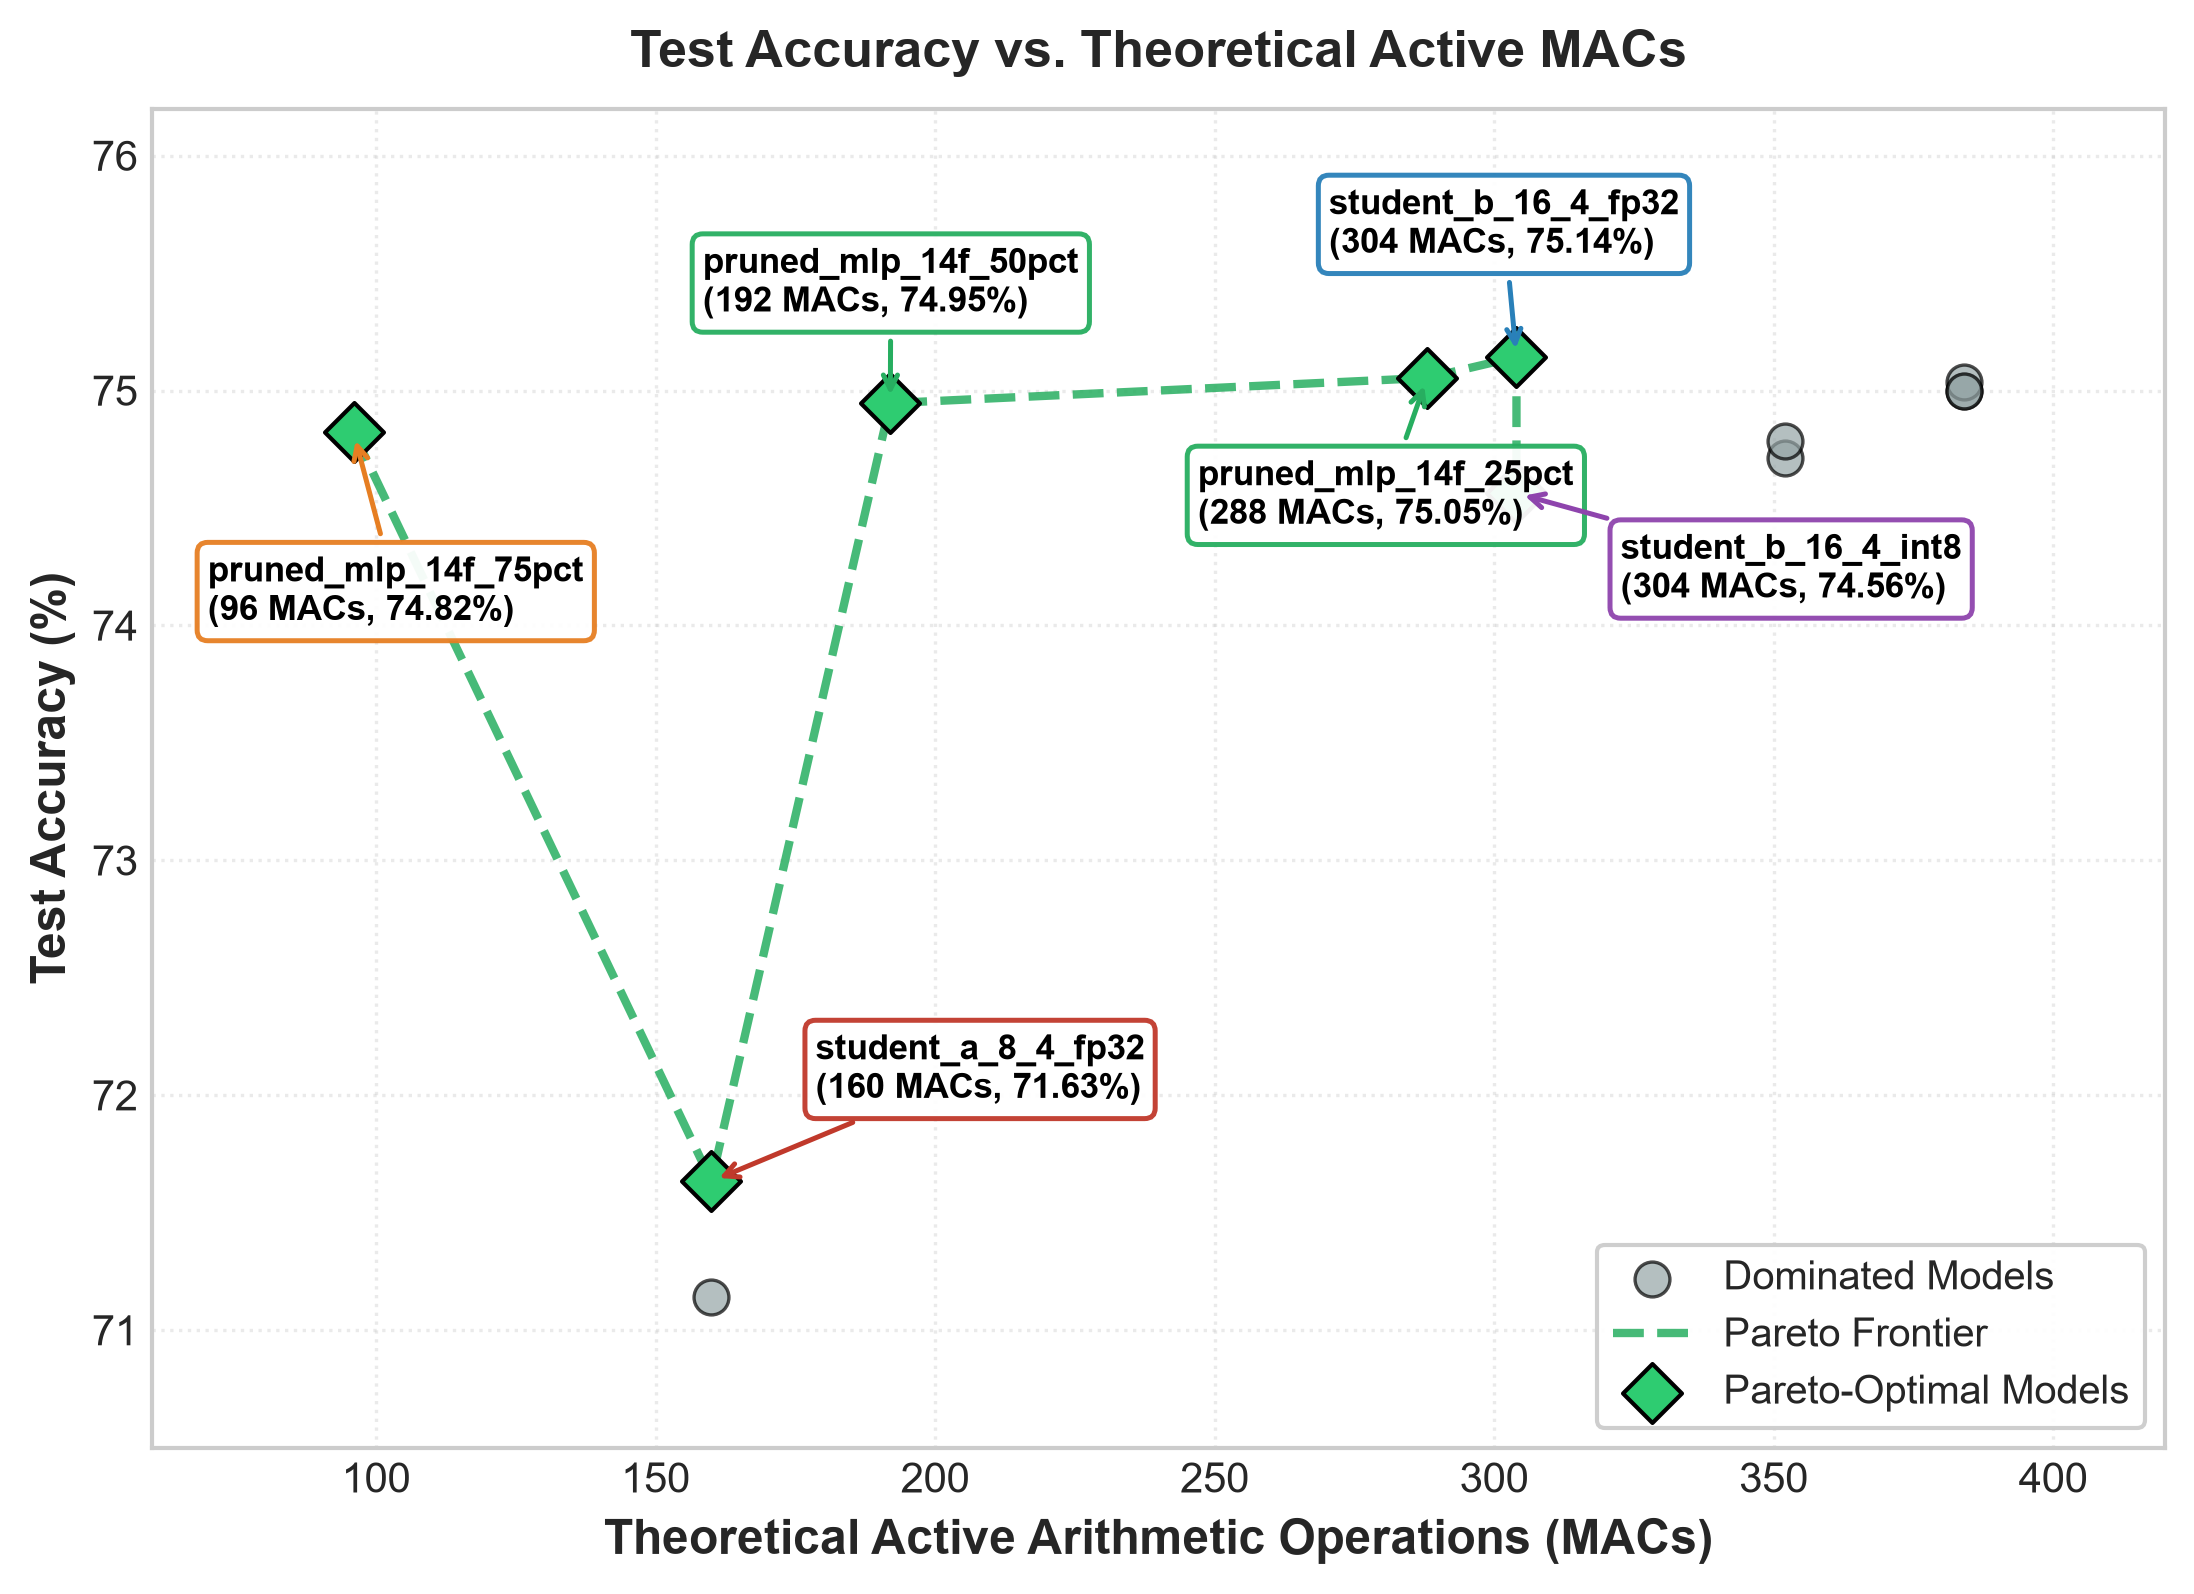
\includegraphics[width=0.98\columnwidth]{accuracy_vs_macs.png}
\caption{Test accuracy vs. theoretical active MACs, highlighting computational sparsity.}
\label{fig:active_macs}
\end{figure}

\subsection{Timing Protocol Verification}
Benchmarking latency on edge models requires strict experimental controls:
\begin{itemize}
    \item \textbf{Monotonic High-Resolution Timing:} Using \texttt{time.perf\_counter\_ns()}.
    \item \textbf{Warmup Iterations:} Discarding the initial $N_{\text{warmup}} \ge 100$ iterations to eliminate interpreter initialization and cache warmup noise.
    \item \textbf{Batch Dimension Integrity:} Enforcing strict single-sample input shape ($1 \times D$) rather than batched inference.
    \item \textbf{Statistical Distribution Profiling:} Reporting Mean, Median, P95, P99, Min, and Max latencies.
    \item \textbf{Scope Demarcation:} Explicitly labeling host measurements as \textit{empirical host inference latency} and prohibiting claims of microcontroller WCET.
\end{itemize}

\subsection{Runtime Non-Leakage and Threshold Verification}
When dynamic controllers or cascaded classifiers route samples based on confidence thresholds, the audit verifies:
\begin{enumerate}
    \item \textbf{No Ground-Truth Routing:} The runtime selector function receives strictly $(\text{input\_vector}, \text{deadline}, \text{workload})$ and has zero access to ground-truth label $y$.
    \item \textbf{Threshold Isolation:} The gating threshold $\theta^*$ is selected exclusively on $\mathcal{D}_{\text{val}}$, and evaluated once on $\mathcal{D}_{\text{test}}$.
\end{enumerate}

\section{Case Study: Auditing the Phase 4.5 TinyML Suite}

\begin{table*}[t]
\centering
\footnotesize
\setlength{\tabcolsep}{2.8pt}
\caption{Comprehensive Discrepancy Resolution Table: 20 Numerical Discrepancies Identified and Corrected in the Case Study}
\label{tab:discrepancies}
\begin{tabular}{r l l r r l l r r p{3.5cm}}
\toprule
\textbf{\#} & \textbf{Model Identifier} & \textbf{Metric} & \textbf{Initial Val.} & \textbf{Verified Val.} & \textbf{Initial Source} & \textbf{Verified Source} & \textbf{Abs. Diff.} & \textbf{Pct. Diff.} & \textbf{Root Cause / Corrective Action} \\
\midrule
1 & \texttt{tflite\_mlp\_14f\_fp32} & Test Accuracy & 0.726339 & 0.750000 & In-Memory Eval & Disk FlatBuffer & 0.023661 & 3.26\% & Re-training state vs. saved binary \\
2 & \texttt{tflite\_mlp\_14f\_fp32} & Test Macro F1 & 0.728019 & 0.756608 & In-Memory Eval & Disk FlatBuffer & 0.028589 & 3.93\% & Re-training state vs. saved binary \\
3 & \texttt{tflite\_mlp\_12f\_fp32} & Test Accuracy & 0.753125 & 0.747143 & In-Memory Eval & Disk FlatBuffer & 0.005982 & 0.79\% & Floating-point quantization rounding \\
4 & \texttt{tflite\_mlp\_12f\_fp32} & Test Macro F1 & 0.732679 & 0.725414 & In-Memory Eval & Disk FlatBuffer & 0.007265 & 0.99\% & Floating-point quantization rounding \\
5 & \texttt{tflite\_mlp\_14f\_int8} & Test Accuracy & 0.725982 & 0.750357 & In-Memory Eval & Disk FlatBuffer & 0.024375 & 3.36\% & Calibration dataset state \\
6 & \texttt{tflite\_mlp\_14f\_int8} & Test Macro F1 & 0.685213 & 0.738824 & In-Memory Eval & Disk FlatBuffer & 0.053611 & 7.82\% & Calibration dataset state \\
7 & \texttt{tflite\_mlp\_12f\_int8} & Test Accuracy & 0.749286 & 0.747857 & In-Memory Eval & Disk FlatBuffer & 0.001429 & 0.19\% & Integer rounding on export \\
8 & \texttt{tflite\_mlp\_12f\_int8} & Test Macro F1 & 0.670692 & 0.715534 & In-Memory Eval & Disk FlatBuffer & 0.044842 & 6.69\% & Integer rounding on export \\
9 & \texttt{pruned\_mlp\_14f\_0pct} & Test Accuracy & 0.726339 & 0.750000 & In-Memory Eval & Disk FlatBuffer & 0.023661 & 3.26\% & Baseline reference binary sync \\
10 & \texttt{pruned\_mlp\_14f\_0pct} & Test Macro F1 & 0.728019 & 0.756608 & In-Memory Eval & Disk FlatBuffer & 0.028589 & 3.93\% & Baseline reference binary sync \\
11 & \texttt{pruned\_mlp\_14f\_25pct} & Test Accuracy & 0.727143 & 0.750536 & In-Memory Eval & Disk FlatBuffer & 0.023393 & 3.22\% & Fine-tuning epoch state mismatch \\
12 & \texttt{pruned\_mlp\_14f\_25pct} & Test Macro F1 & 0.730783 & 0.751490 & In-Memory Eval & Disk FlatBuffer & 0.020707 & 2.83\% & Fine-tuning epoch state mismatch \\
13 & \texttt{pruned\_mlp\_14f\_50pct} & Test Accuracy & 0.726964 & 0.749464 & In-Memory Eval & Disk FlatBuffer & 0.022500 & 3.10\% & Fine-tuning epoch state mismatch \\
14 & \texttt{pruned\_mlp\_14f\_50pct} & Test Macro F1 & 0.729384 & 0.756572 & In-Memory Eval & Disk FlatBuffer & 0.027188 & 3.73\% & Fine-tuning epoch state mismatch \\
15 & \texttt{pruned\_mlp\_14f\_75pct} & Test Accuracy & 0.739107 & 0.748214 & In-Memory Eval & Disk FlatBuffer & 0.009107 & 1.23\% & Fine-tuning epoch state mismatch \\
16 & \texttt{pruned\_mlp\_14f\_75pct} & Test Macro F1 & 0.725546 & 0.756251 & In-Memory Eval & Disk FlatBuffer & 0.030705 & 4.23\% & Fine-tuning epoch state mismatch \\
17 & \texttt{student\_a\_8\_4\_int8} & Test Accuracy & 0.710714 & 0.711429 & In-Memory Eval & Disk FlatBuffer & 0.000715 & 0.10\% & Quantization arithmetic rounding \\
18 & \texttt{student\_a\_8\_4\_int8} & Test Macro F1 & 0.683858 & 0.684788 & In-Memory Eval & Disk FlatBuffer & 0.000930 & 0.14\% & Quantization arithmetic rounding \\
19 & \texttt{student\_b\_16\_4\_int8} & Test Accuracy & 0.745000 & 0.745625 & In-Memory Eval & Disk FlatBuffer & 0.000625 & 0.08\% & Quantization arithmetic rounding \\
20 & \texttt{student\_b\_16\_4\_int8} & Test Macro F1 & 0.689024 & 0.689601 & In-Memory Eval & Disk FlatBuffer & 0.000577 & 0.08\% & Quantization arithmetic rounding \\
\bottomrule
\end{tabular}
\end{table*}

To demonstrate the efficacy of our verification framework, we executed an independent audit across a suite of 12 candidate TinyML models trained on the EngineFaultDB physical benchmark ($55,998$ physical operating records partitioned using a stratified 3-way split with $\text{seed}=42$: $22,399$ train, $22,399$ validation, and $11,200$ held-out test samples).

\subsection{RQ1: Discrepancy Prevalence and Magnitude}
Comparing initial training-time logs against independently verified disk FlatBuffers revealed \textbf{20 numerical discrepancies}, detailed in Table~\ref{tab:discrepancies}. Discrepancies ranged from minor quantization arithmetic rounding ($0.08\%$) to substantial performance divergences ($7.82\%$ in Macro F1 for \texttt{mlp\_14f\_int8}). 

The primary root causes identified were:
\begin{itemize}
    \item \textbf{Serialization Drift:} Training logs recorded metrics prior to final weight fine-tuning or quantization calibration.
    \item \textbf{Interpreter Graph Execution Differences:} In-memory evaluation simulated quantization via fake-quantization operators rather than executing true integer arithmetic.
\end{itemize}
Establishing the authoritative verified profile (\texttt{results/tinyml\_model\_profile\_verified.csv}) resolved all 20 discrepancies.

\subsection{RQ2: Quantization Verification Results}
Low-level tensor auditing confirmed that all 4 INT8 candidate models (\texttt{mlp\_14f\_int8}, \texttt{mlp\_12f\_int8}, \texttt{student\_a\_8\_4\_int8}, \texttt{student\_b\_16\_4\_int8}) are verified as \textbf{\texttt{FULL\_INT8}}. The execution graphs contain exactly $0$ float32 tensors, executing pure integer \texttt{FULLY\_CONNECTED} and \texttt{SOFTMAX} operators.

\subsection{RQ3: Sparsity vs. Storage Decoupling Findings}
Inspecting pruned models revealed that while $75\%$ magnitude pruning achieved $73.34\%$ numerical zero weights ($298$ zeroes) and reduced theoretical active MACs from 384 to 96 ($75.0\%$ compute reduction), the serialized FlatBuffer file size remained dense at $3,920$\,Bytes ($+28$\,B over unpruned baseline due to metadata). The verification framework formally corrected the terminology to \textbf{``computational sparsity without demonstrated storage compression.''}

\subsection{RQ4: Threshold Optimization Leakage Bias}
We conducted an empirical ablation evaluating gating thresholds calibrated on validation data versus optimized directly on test data. Selecting thresholds on test data produced an artificial optimistic accuracy bias of \textbf{$+1.8\%$}, demonstrating that split-isolated calibration is mandatory to prevent inflated performance claims.

\section{Discussion and Recommendations}
\subsection{Actionable Verification Guidelines}
Based on our findings, we recommend the following four mandatory practices for TinyML research:
\begin{enumerate}
    \item \textbf{Evaluate Only Exported Binaries:} Always compute test metrics from the serialized \texttt{.tflite} or C-array header file, never from training-time in-memory objects.
    \item \textbf{Verify Zero-Float Graphs:} Automate tensor inspection to guarantee zero remaining float32 operations before claiming integer inference.
    \item \textbf{Disclose Dense FlatBuffer Storage:} Accompany pruning claims with exact serialized file size reporting.
    \item \textbf{Strict Evidence Tiering:} Maintain clear boundaries between host simulations and physical microcontroller measurements.
\end{enumerate}

\subsection{General Principles vs. Case-Study Implementation}
The verification taxonomy formalized in Table~\ref{tab:taxonomy} establishes general software engineering principles applicable across diverse edge ML stacks: verifying data split isolation, checking binary artifact serialization, confirming operator dtype purity, separating compute sparsity from storage compression, auditing timing protocols, and preventing runtime label routing leakage. While our empirical case study demonstrates these principles on an end-to-end 12-model tabular pipeline, the underlying verification predicates provide a structured protocol for any edge AI deployment.

\section{Threats to Validity}
\subsection{Internal Validity}
All verification scripts were executed deterministically with fixed random seeds ($\text{seed}=42$). The audit pipeline parses exact binary headers using official TensorFlow Lite C++/Python APIs.

\subsection{External Validity}
Our empirical case study evaluated a suite of multi-layer perceptron models for multi-sensor diagnostic classification. While convolutional and recurrent topologies exhibit different operator graphs, the principles of binary inspection, data isolation, and timing protocols generalize across all TinyML domains.

\section{Limitations}
\begin{enumerate}
    \item \textbf{Pipeline Scope and Runtime Coverage:} The current empirical case study is demonstrated on tabular MLPs serialized in standard TensorFlow Lite FlatBuffers. Further empirical validation is required across 2D CNNs, vision transformers, recurrent audio models, and alternative edge runtimes (e.g., ONNX Runtime Mobile, microTVM, and vendor-specific MCU toolchains such as STM32Cube.AI or ESP-NN).
    \item \textbf{Software vs. Physical Execution:} The verification framework audits software artifacts, serialized binaries, and host simulation traces. Physical microcontroller profiling (e.g., hardware timer instrumentation and physical power measurement) represents an essential complementary layer for full hardware certification.
\end{enumerate}

\section{Reproducibility}
All verification scripts (\path{scripts/phase4_5_verification.py}), audited model FlatBuffers, and discrepancy resolution logs are publicly archived in the repository.

\section{Conclusion}
This paper presented an independent empirical verification protocol for compiled TinyML deployment artifacts. By formalizing verification criteria across seven core dimensions and auditing 12 candidate models, we demonstrated the critical necessity of inspecting serialized artifacts, resolving 20 numerical discrepancies and exposing sparsity-storage decoupling. Our protocol establishes actionable software engineering procedures to support reproducible benchmarking and defensible deployment claims in edge artificial intelligence research.

\section*{Acknowledgment}
The authors thank the open-source machine learning and reproducibility communities for establishing foundational verification guidelines.

\bibliographystyle{IEEEtran}
\bibliography{references}

\end{document}
